\renewcommand{\theequation}{\theenumi}
\begin{enumerate}[label=\arabic*.,ref=\thesubsection.\theenumi]
\numberwithin{equation}{enumi}
\item In a certain test, $a_i$ students gave wrong answers to atleast i questions, where $i = 1,2,...,k.$ No student gave more than k wrong answers. The total number of wrong answers given is.....\\
\item The side AB, BC and CA of a triangle ABC have 3, 4 and 5 interior points respectively on them. The number of triangles that can be constructed using these interior points as vertices is.....\\
\item Total number of ways in which six $'+'$ and four $'-'$ signs can be arranged in a line such that no two $'-'$ signs occur together is......\\
\item There are four balls of different colours and four boxes of colours, same as those of the balls. The number of ways in which the balls, one each in a box, could be placed such that a ball does not go to a box of its own colour is.....\\
\item The product of any r consecutive natural numbers is always divisible by r!\\
\item $\nCr{n}{r-1} = 36$, $\nCr{n}{r} = 84$ and $\nCr{n}{r+1} = 126$, then r is :
\begin{enumerate}
\item 1
\item 2
\item 3
\item None of these.\\
\end{enumerate}
\item Ten different letters of an alphabet are given. Words with five letters are formed from these given letters. Then the number of words which have at least one letter repeated are
\begin{enumerate}
\item 69760
\item 30240
\item 99748
\item none of these\\
\end{enumerate}
\item The value of the expression $\nCr{47}{4}+\sum_{j=1}^{5} \nCr{52-j}{3}$ is equal to
\begin{enumerate}
\item $\nCr{47}{5}$
\item $\nCr{52}{5}$
\item $\nCr{52}{4}$
\item none of these\\
\end{enumerate} 
\item Eight chairs are numbered 1 to 8. Two women and three men wish to occupy one chair each. First the women choose the chairs from amongst the chairs marked 1 to 4; and then the men select the chairs from amongst the remaining. The number of possible arrangments is
\begin{enumerate}
\item $\nCr{6}{3}$ $\times$ $\nCr{4}{2}$
\item $\\nPr{4}{2}$ $\times$ $\\nPr{4}{3}$
\item $\nCr{4}{2}$ + $\\nPr{4}{3}$
\item none of these\\
\end{enumerate}
\item A five-digit numbers divisible by 3 is to be formed using the numerals 0, 1, 2, 3, 4 and 5, without repetition. The total number of ways this can be done is
\begin{enumerate}
\item 216
\item 240
\item 600
\item 3125\\
\end{enumerate}
\item How many different nine digit numbers can be formed from the number 223355888 by rearranging its digits so that the odd digits occupy even positions?
\begin{enumerate}
\item 16
\item 36
\item 60
\item 180\\
\end{enumerate}
\item Let $T_n$ denote the number of triangles which can be formed using the vertices of a regular polygon of n sides. If $T_{n+1}-T_n = 21$, then n equals
\begin{enumerate}
\item 5
\item 7
\item 6
\item 4\\
\end{enumerate}
\item The number of arrangements of the letters of the word BANANA in which the two N's do not apppear adjacently is
\begin{enumerate}
\item 40
\item 60
\item 80
\item 100\\
\end{enumerate}
\item A rectangle with sides of length (2m-1) and (2n-1) units is divided into squares of unit length by drawing parallel lines as shown in the diagram, then the number of rectangles possible with odd side lengths is
\begin{figure}
	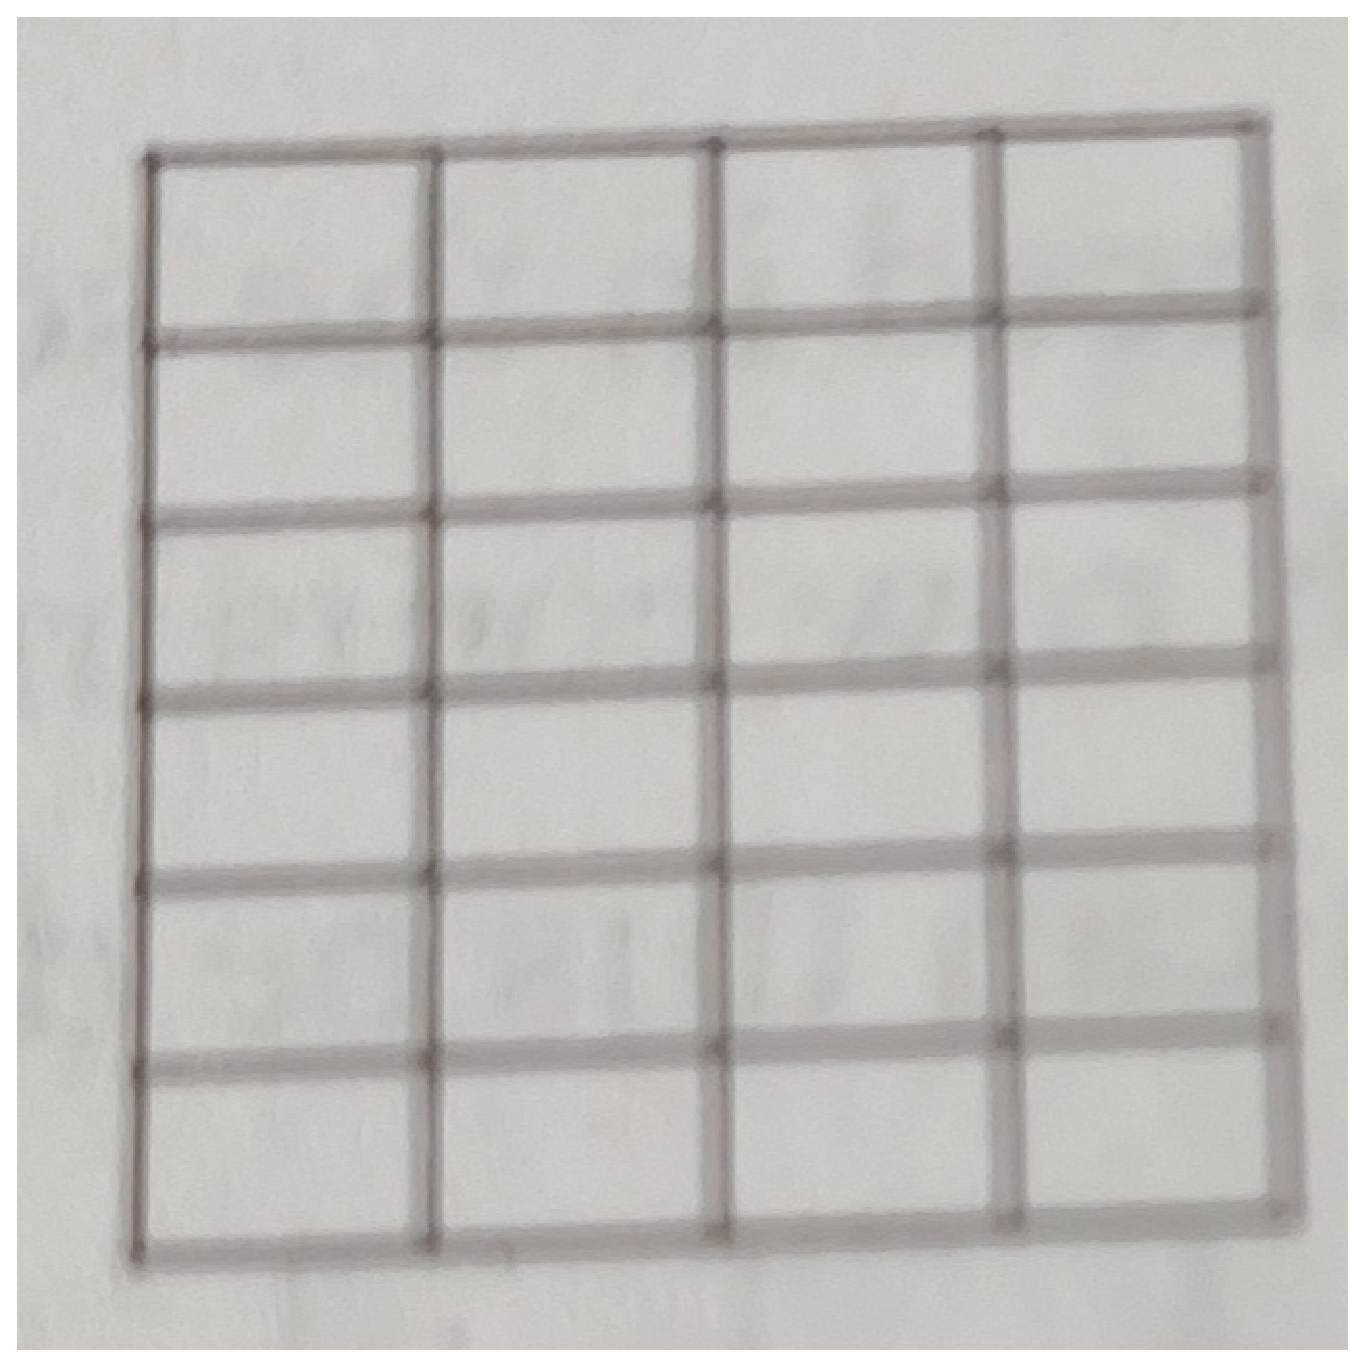
\includegraphics[width=30mm,scale=0.5]{./figs/a.eps} 
\end{figure}
\begin{enumerate}
\item $(m+n-1)^2$
\item $4^{m+n-1}$
\item $m^2n^2$
\item $m(m+1)n(n+1)$\\
\end{enumerate}
\item If the LCM of p, q is $r^2t^4s^2$, where r, s, t are prime numbers and p,q are the positive integers then the number of ordered pair $(p,q)$ is
\begin{enumerate}
\item 252
\item 254
\item 225
\item 224\\
\end{enumerate}
\item The letters of the word COCHIN are computed and all the computations are arranged in an alphabetical order as in an English dictionary. The number of words that appear before the word COCHIN is 
\begin{enumerate}
\item 360
\item 192
\item 96
\item 48\\
\end{enumerate}
\item The number of seven digit integers, with sum of the digits equal to 10 and formed by using the digits 1,2 and 3 only, is
\begin{enumerate}
\item 55
\item 66
\item 77
\item 88\\
\end{enumerate}
\item The total number of ways in which 5 balls of different colours can be distributed among 3 persons so that each person gets at least one ball is 
\begin{enumerate}
\item 75
\item 150
\item 210
\item 243\\
\end{enumerate}
\item Six cards and six envelopes are numbered 1,2,3,4,5,6 and cards are to be placed in envelopes so that each envelope contains exactly one card and no card is placed in the envelope bearing the same number and moreover the card numbered 1 is always placed in envelope numbered 2. Then the number of ways it can be done is 
\begin{enumerate}
\item 264
\item 265
\item 53
\item 67\\
\end{enumerate} 
\item A Debate club consists of 6 girls and 4 boys. A team of 4 members is to be selected from this club including the selection of a captain (from among these 4 members) for the team. If the team has to include  at most one boy, then the number of ways of selecting the team is 
\begin{enumerate}
\item 380
\item 320
\item 260
\item 95\\
\end{enumerate}
\item An n-digit number is a positive number with exactly n digits. Nine hundred distinct n-digit numbers are to be formed using only three digits 2,5 and 7. The smallest value of n for which this is possible is
\begin{enumerate}
\item 6
\item 7
\item 8
\item 9\\
\end{enumerate}
\item Six X's have to be placed in the sqaures of figure given below in such a way that each row contains atleast one X. In how many different ways can this be done
\begin{figure}
	\includegraphics[width=30mm,scale=0.5]{./figs/b.eps} 
\end{figure}\\
\item Five balls of different colours are to be placed in the boxes of different size. Each box can hold all five. In how many different ways can we place the balls so that no box remains empty?\\
\item m men and n women are to be seated in a row so that no two women sit together. If $m>n$, then show that the number of ways in which they can be seated is $\frac{m!(m+1)!}{(m-n+1)!}$\\
\item 7 relatives of a man comprises 4 ladies and 3 gentlemen; his wife also has 7 relatives; 3 of them are ladies and 4 gentlemen. In how many ways they can invite a dinner party of 3 ladies and 3 gentlemen so that there are 3 of man's relatives and 3 of wife's relatives?\\
\item A box contains two white balls, three black balls, four red balls. In how many ways can three balls be drawn from the box if at least one black ball is to be included in the draw?\\
\item Eighteen guests have to be seated, half on each side of a long table. Four particular guests desire to sit on one particular side and three others on the others side. Determine the number of ways in which the sitting arragements can be made.\\
\item A committee of 12 is to be formed from 9 women and 8 men.In how many ways this can be done if at least five women have to be included in a committee? In how many of these committees
\begin{enumerate}
\item The women are in majority?
\item The men are in majority?\\
\end{enumerate}
\item Prove by computation or otherwise $\frac{(n^2)!}{(n!)^n}$ is an integer $(n\epsilon I^+)$.\\
\item If total number of runs scored in n matches is $(\frac{n+1}{4})$ $(2^{n+1}-n-2)$ where $n>1$, and the runs scored in the kth match are given by K. $2^{n+1-k}$, where $1\leq k\leq n.$ Find n.\\

Let $a_n$ denote the number of all n-digit positive integers formed by the digits 0, 1 or both such that no consecutive digits in them are 0. Let $b_n=$ the number of such n-digit integers ending with digit 1 and $c_n=$ the number of such n-digit integers ending with digit 0.\\
\item The value of $b_6$ is
\begin{enumerate}
\item 7
\item 8
\item 9
\item 11\\
\end{enumerate}
\item which of the following is correct?
\begin{enumerate}
\item $a_{17} = a_{16} + a_{15}$
\item $c_{17} \neq c_{16} + c_{15}$
\item $b_{17} \neq b_{16} + c_{16}$
\item $a_{17} = c_{17} + b_{16}$\\
\end{enumerate}
\item Consider the set of eight vectors V=$\lbrace$a\^{i}+b\^{j}+c\^{k}:a,b,c$\epsilon\lbrace-1,1\rbrace$ $\rbrace.$ Three non-coplanar vectors can be chosen from V in $2^p$ ways. Then p is\\

\item Let $n_1<n_2<n_3<n_4<n_5$ be positive integers such that $n_1+n_2+n_3+n_4+n_5=20.$ Then the number of such distinct arrangements $(n_1,n_2,n_3,n_4,n_5)$ is\\
\item Let $n\geq2$ be an integer. Take n distinct points on a circle and join each pair of points by a line segment. Colour the line segment by joining every pair of adjacent points by blue and the rest by red. If the number of red and blue line segments are equal, then the value of n is\\
\item Let n be number of ways in which 5 boys and 5 girls can stand in a queue in such a way that all the girls stand consecutively in the queue. Let m be the number of ways in which 5 boys and 5 girls can stand in a queue in such a way that exactly four girls stand consecutively in the queue. Then the value of $\frac{m}{n}$ is\\
\item Words of length 10 are formed using the letters A, B, C, D, E, F, G, H, I, J. Let x be the number of such words where no letter is repeated; and let y be the number of such words where exactly one letter is repeated twice and no other letter is repeated. Then, $\frac{y}{9x} = $\\
\item The number of 5 digit numbers which are divisible by 4, with digits from the set $\left\lbrace1,2,3,4,5\right\rbrace$ and the repetition of digits is allowed, is\\
\item Let $\vert X \vert$ denote the number of elements in a set X. Let S$=\left\lbrace1,2,3,4,5,6\right\rbrace$ be a sample space, where each element is likely to occur. If A and B are independent events associated with S, then the number of ordered pairs (A,B) such that $1\leq\vert B \vert < \vert A \vert$, equals.\\
\item Five persons A, B, C, D and E are seated in a circular arrangement. If each of them is given a hat of one of the three colours red, blue and green, then the number of ways of distributing the hats such that the persons seated in adjacent seats get different coloured hats is...\\ 
\item Total no of four digit odd numbers that can be formed using 0,1,2,3,5,7 (using the repetition allowed) are
\begin{enumerate}
\item 216
\item 375
\item 400
\item 720
\end{enumerate}
\item Number greater than 1000 but less than 4000 is formed using the digits 0,1,2,3,4 (repetition allowed). Their number is 
\begin{enumerate}
\item 125
\item 105 
\item 375
\item 625\\
\end{enumerate}
\item Five digit number divisible by 3 is formed using 0,1,2,3,4 and 5 without repetition. Total number of such numbers are
\begin{enumerate}
\item 312
\item 3125 
\item 120
\item 216\\
\end{enumerate}
\item The sum of integers from 1 to 100 that are divisible by 2 or 5 is
\begin{enumerate}
\item 3000
\item 3050
\item 3600
\item 3250\\
\end{enumerate}
\item If $\nCr{n}{r}$ denotes the number of combination of n things taken r at a time, then the expression $\nCr{n}{r+1}+\nCr{n}{r-1}+2 \times \nCr{n}{r}$ equals
\begin{enumerate}
\item $\nCr{n+1}{r+1}$
\item $\nCr{n+2}{r}$
\item $\nCr{n+2}{r+1}$
\item $\nCr{n+1}{r}$\\
\end{enumerate}
\item A student is to answer 10 out of 13 questions in an examination such that he must choose at least 4 from the first five questions. The number of choices available to him is
\begin{enumerate}
\item 346
\item 140 
\item 196
\item 280\\
\end{enumerate}
\item The number of ways in which 6 men and 5 women can dine at a round table if no two women are to sit together is given by
\begin{enumerate}
\item $7! \times 5!$
\item $6! \times 5!$
\item 30!
\item $5! \times 4!$\\
\end{enumerate}
\item How many ways are there to arrange the letters in the word GARDEN with vowels in alphabetical order
\begin{enumerate}
\item 480
\item 240 
\item 360
\item 120\\
\end{enumerate}
\item The number of ways of distributing 8 identical balls in 3 distinct boxes so that none of the boxes is empty is 
\begin{enumerate}
\item $\nCr{8}{3}$
\item 21
\item $3^8$
\item 5\\
\end{enumerate}
\item If the letters of the word SACHIN are arranged in all possible ways and these words are written out as in dictionary, then the word SACHIN appears at serial number
\begin{enumerate}
\item 601
\item 600 
\item 603
\item 602\\
\end{enumerate}
\item At an election, a voter may vote for any number of candidates, not greater than the number to be elected. There are 10 candidates and 4 are to be selected, if a voter votes for at least one candidate, then the number of ways in which he can vote is
\begin{enumerate}
\item 5040
\item 6210 
\item 385
\item 1110\\
\end{enumerate} 
\item The set S $= \left\lbrace1,2,3.....12\right\rbrace$ is to be partitioned into three sets A, B, C of equal size. Thus $A \cup B \cup C = S$, $A \cap B=B \cap C=A \cap C= \phi$. The number of ways to partition S is 
\begin{enumerate}
\item $\frac{12!}{(4!)^3}$
\item $\frac{12!}{(4!)^4}$
\item $\frac{12!}{3!(4!)^3}$
\item $\frac{12!}{3!(4!)^4}$\\
\end{enumerate} 
\item In a Shop there are five types of icecreams available. A child buys six ice-creams.
Statement-1 : The number of different ways the child can buy the six ice-creams is $\nCr{10}{5}$.
Statement-2 : The number of different ways the child can but the six ice-creams is equal to the number of different ways of arranging 6 A's and 4 B's in a row.
\begin{enumerate}
\item Statement-1 is False, Statement-2 is True
\item Statement-1 is True, Statement-2 is True; Statement-2 is a correct explanation for Statement-1
\item Statement-1 is True, Statement-2 is True; Statement-2 is not a correct explanation for Statement-1
\item Statement-1 is True, Statement-2 is False\\ 
\end{enumerate}
\item How many different words can be formed by jumbling the letters in the word MISSISSIPPI in which no two S are adjacent?
\begin{enumerate}
\item $8.\nCr{6}{4}.\nCr{7}{4}$
\item $6.7.\nCr{8}{4}$
\item $6.8.\nCr{7}{4}$
\item $7.\nCr{6}{4}.\nCr{8}{4}$\\
\end{enumerate}   
\item From 6 different novels and 3 different ditionaries, 4 novels and 1 dictionary are to be selected and arranged in a row on a shelf so that the dictionary is always in the middle. Then the number of such arrangement is :
\begin{enumerate}
\item at least 500 but less than 750
\item at least 750 but less than 1000
\item at least 1000
\item at least 500\\ 
\end{enumerate}
\item There are two urns. Urn A has 3 distinct red balls and Urn B has 9 distinct blue balls. From each urn two balls are taken out at random and then transferred to the other. The number of ways in which this can be done is
\begin{enumerate}
\item 36
\item 66 
\item 108
\item 3\\
\end{enumerate}
\item Statement-1 :  The number of ways of distributing 10 identical balls in 4 distinct boxes such that no box is empty is $\nCr{9}{3}$.
Statement-2 : The number of ways of choosing any 3 places from 9 different places is $\nCr{9}{3}$.
\begin{enumerate}
\item Statement-1 is True, Statement-2 is True; Statement-2 is not a correct explanation for Statement-1
\item Statement-1 is True, Statement-2 is False
\item Statement-1 is False, Statement-2 is True
\item Statement-1 is True, Statement-2 is True; Statement-2 is a correct explanation for Statement-1\\
\end{enumerate} 
\item These are 10 points in a plane, out of these 6 are collinear, if N is the number of triangles formed by joining these points. then:
\begin{enumerate}
\item $n \leq 100$
\item $100 < n \leq 140$
\item $140 < n \leq 190$
\item $n > 190$\\
\end{enumerate}  
\item Assuming the balls to be identical except for difference in colours, the number of ways in which one  or more balls can be selected from 10 white, 9 green, and 7 black balls is :
\begin{enumerate}
\item 880
\item 629
\item 630
\item 879\\
\end{enumerate}
\item Let $T_n$ be the number of all possible traingles formed by joining vertices of an n-sided regular polygon. If $T_{n+1}-T_n = 10$, then the value of n is:
\begin{enumerate}
\item 7
\item 5
\item 10
\item 8\\
\end{enumerate}
\item The number of integers greater than 6000 that can be formed, using the digits 3, 5, 6, 7 and 8, without repetition, is :
\begin{enumerate}
\item 120
\item 72
\item 216
\item 192\\
\end{enumerate}
\item If all the words (with or without meaning) having five letters, formed using the letters of the word SMALL and arranged as in a dictionary; then the position of the word SMALL is :
\begin{enumerate}
\item $52^{nd}$
\item $58^{th}$
\item $46^{th}$
\item $59^{th}$\\
\end{enumerate}
\item A man X has 7 friends, 4 of them are ladies and 3 are men. His wife Y also has 7 friends, 3 of them are ladies and 4 are men. Assume X and Y have no common friends. Then the total number of ways in which X and Y together can throw a party inviting 3 ladies and 3 men, so that 3 friends of each of X and Y are in this party, is :
\begin{enumerate}
\item 484
\item 485
\item 468
\item 469\\
\end{enumerate}
\item From 6 different novels and 3 different dictionaries; 4 novels and 1 dictionary are to be selected and arranged in a row on a shelf so that the dictionary is always in the middle. The number of such arrangements is :
\begin{enumerate}
\item less than 500
\item at least 500 but less than 750
\item at least 750 but less than 1000
\item at least 1000\\ 
\end{enumerate}
\item Consider a class of 5 girls and 7 boys. The number of different teams consisting of 2 girls and 3 boys that can be formed from this class, if there are two specific boys A and B, who refuse to be the members of the same team, is:
\begin{enumerate}
\item 500
\item 200
\item 300
\item 350\\
\end{enumerate} 
\item A committee of 11 members is to be formed from 8 males and 5 females. If m is the number of ways the committee is formed with at least 6 males and n is the number of ways the committee is formed with at least 3 females, then:
\begin{enumerate}
\item m + n = 68
\item m = n = 78
\item n = m - 8
\item m = n = 68\\
\end{enumerate}


Each question contains statements given in two columns, which have to be matched. The statements in Column-I are labelled A, B, C, D, while the statements in Column-II are labelled p, q, r, s and t. Any given statement in Column-I can have correct matching with ONE OR MORE statements in Column-II. The appropriate bubbles corresponding to the answers to these questions have to be darkened as illustrated in the following example :
If the correct matches are A-p, s and t; B-q and r; C-p and q; and D-s, then the correct darkening of bubbles will look like

\begin{figure}
	\includegraphics[width=30mm,scale=0.5]{./figs/c.eps} 
\end{figure}
%
\item Consider all possible computations of the letters of the word ENDEANOEL. Match the Statements/Expressions in Column-I with the Statements/Expressions in column-II and indicate your answer by darkening the appropriate bubbles in the $4 \times 4$ matrix given in the ORS.\\
\resizebox{\columnwidth}{14pt}{%
\begin{tabular}{cc}
Column-I &Column-II\\
(A) The number of computations containing the word ENDEA is&(p)5!\\
(B) The number of computations in which the letter E occurs in the first and the last positions is&(q)2 $\times$ 5!\\ 
(C) The number of computations in which none of the letters D, L, N occurs in the last five positions is&(r)7 $\times$ 5!\\
(D) The number of computations in which the letters A, E, O occur only in odd positions is&(s)21 $\times$ 5!\\
\end{tabular}}\\


\item In a high school, a committe has to be formed from a group of 6 boys $M_1,M_2,M_3,M_4,M_5,M_6$ and 5 girls $G_1,G_2,G_3,G_4,G_5.$
\begin{enumerate}
\item Let $\alpha_1$ be the total number of ways in which the committe can be formed such that the committe has 5 members, having exactly 3 boys and 2 girls.
\item Let $\alpha_2$ be the total number of ways in which the committe can be formed such that the committe has at least 2 members and having an equal number of boys and girls.
\item Let $\alpha_3$ be the total number of ways in which the committe can be formed such that the committe has 5 members at least 2 of them being girls.
\item Let $\alpha_4$ be the total number of ways in which the committe can be formed such that the committe has 4 members, having at least 2 girls and such that both $M_1$ and $G_1$ are NOT in the committe together.
\end{enumerate}
\begin{table}[h!]
\centering
\begin{tabular}{c c} 
 LIST-I & LIST-II\\ [0.5ex] 
 P. The value of $\alpha_1$ is & 1. 136 \\ 
 Q. The value of $\alpha_2$ is & 2. 189\\
 R. The value of $\alpha_3$ is & 3. 192\\
 S. The value of $\alpha_4$ is & 4. 200\\
 & 5. 381\\
 & 6. 461\\ [1ex] 
\end{tabular}
\end{table}
The correct option is:\\
\begin{enumerate}
\item P$\rightarrow$4; Q$\rightarrow$6; R$\rightarrow$2; S$\rightarrow$1
\item P$\rightarrow$1; Q$\rightarrow$4; R$\rightarrow$2; S$\rightarrow$3
\item P$\rightarrow$4; Q$\rightarrow$6; R$\rightarrow$5; S$\rightarrow$2
\item P$\rightarrow$4; Q$\rightarrow$2; R$\rightarrow$3; S$\rightarrow$1
\end{enumerate}

\end{enumerate}
